\documentclass[a4paper,12pt,french] {article}

\usepackage[TD]{../../../Style}

%\usepackage{fancyhdr}
%\usepackage[french]{babel}
%\usepackage[margin=2cm]{geometry}
\pagestyle{empty}

\definecolor{couleurTriangle}{Hsb}{211,0.8,0.65}
\newcommand{\exoTriangle}{\textcolor{couleurTriangle}\blacktriangleright \ } 

\usetikzlibrary{intersections}

\usepackage{tkz-euclide}

\setstretch{1.3}

% Doc repris de l'APMEP

\begin{document}

\titre{Les dents vertes}

Voici une liste d'énoncés. Chacun d'eux sera considéré comme vrai, même s'il paraît absurde.

\vspace{5mm}
%\noindent
%\textit{Chaque propriété qui suit est considérée comme vrai.}\\

\noindent
\textbf{E1} \: :
\textit{S'il fait beau, alors les jeunes vont se promener.}

\noindent
\textbf{E2} \: :
\textit{Si des poules chantent, alors elles ont les dents vertes.}

\noindent
\textbf{E3} \: :
\textit{S'il fait nuit, alors les chats sont gris.}

\noindent
\textbf{E4} \: :
\textit{Si un jeune a de l'argent et passe devant une pâtisserie, alors il s'achète des petits gâteaux.} 

\noindent
\textbf{E5} \: :
\textit{Si un jeune a des caries, alors il va chez le dentiste.}

\noindent
\textbf{E6} \: :
\textit{Si un jeune chante à tue-tête, alors ses voisins sont contents.}

\noindent
\textbf{E7} \: :
\textit{Si un jeune fait des mathématiques, alors c'est le bonheur absolu !}

\noindent
\textbf{E8} \: :
\textit{Si un jeune fait du sport, alors il transpire.}

\noindent
\textbf{E9} \: :
\textit{Si un jeune mange des sucreries, alors il a des caries.}

\noindent
\textbf{E10} :
\textit{Si un jeune se couche tard, alors il est fatigué.}

\noindent
\textbf{E11} :
\textit{Si un jeune se douche, alors il met de l'eau partout dans la salle de bain.}

\noindent
\textbf{E12} :
\textit{Si un jeune se douche, alors il est propre.}

\noindent
\textbf{E13} :
\textit{Si un jeune met de l'eau partout dans une pièce, alors il doit nettoyer les sols}.

\noindent
\textbf{E14} :
\textit{Si un jeune sort de chez lui, alors il passe devant la pâtisserie.}

\noindent
\textbf{E15} :
\textit{Si un jeune transpire, alors il se douche.}

\noindent
\textbf{E16} :
\textit{Si un jeune est fatigué, alors il s'endort sur son bureau.}

\noindent
\textbf{E17} :
\textit{Si un jeune travaille bien, alors il reçoit de l'argent de poche.}

\noindent
\textbf{E18}:
\textit{Si les voisins sont heureux et que les chats sont gris, alors les poules chantent la Marseillaise.}

\vspace{10mm}

\begin{exercice}
Jeudi dernier, Nadia a trop fait la fête, et elle s'est couchée tard.

\exoTriangle Démontrer qu'elle va s'endormir sur son bureau.
\end{exercice}

\begin{exercice}
Dimanche, Pierre a fait du sport (il a joué au football) tout l'après-midi. Son équipe a gagné sur le score de 3 - 0.

\exoTriangle Démontrer qu'il va nettoyer les sols de la salle de bain.
\end{exercice}

\begin{exercice}
La nuit est tombée et Carole va se coucher.
Comme elle ne trouve pas le sommeil, elle ouvre la fenêtre, branche son baladeur et écoute de la musique en observant les étoiles. Avec son casque sur les oreilles, elle ne se rend pas compte qu'elle chante très fort.

\exoTriangle Démontrer que les poules ont les dents vertes.
\end{exercice}

\begin{exercice}
Nous sommes lundi, il est 10 heures et le soleil brille.
Léo est heureux, car il a bien travaillé et a reçu un 18/20 en français.

\exoTriangle Démontrer qu'il va aller chez le dentiste.
\end{exercice}

\begin{exercice}[*]
Damien n'a pas de caries.

\exoTriangle Montrer que soit Damien ne travaille pas bien, soit il ne fait pas beau.
\end{exercice}

\begin{exercice}[*]
Les poules ne chantent pas la Marseillaise.

\exoTriangle Que peut-on en déduire?
\end{exercice}

\newpage

\begin{exercice}
A partir des propriétés codées sur la figure et de certains théorèmes de la liste ci-dessous, démontrer que le quadrilatère $ABCD$ est un parallélogramme.

\vspace{1cm}

\begin{center}
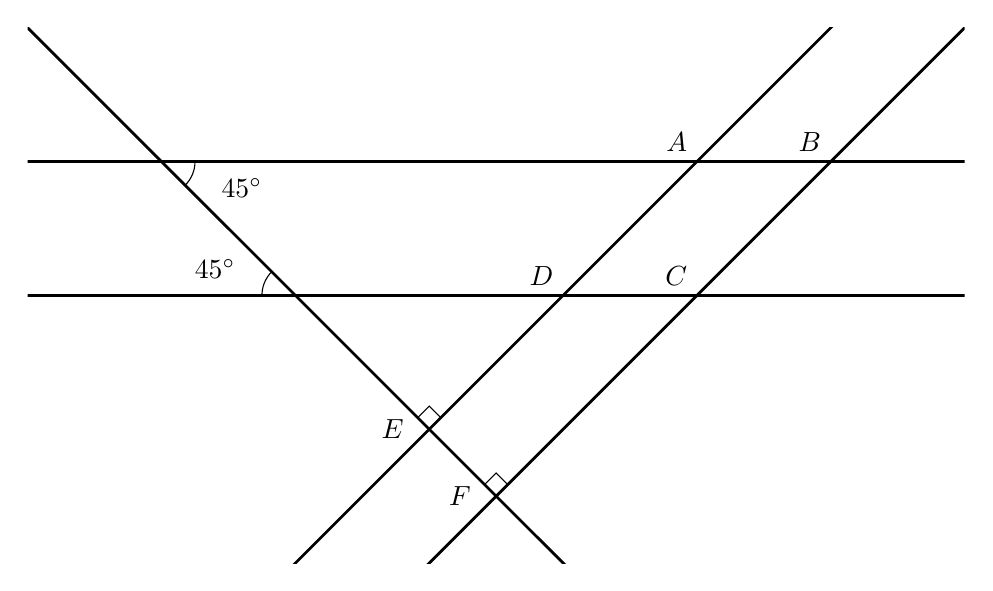
\begin{tikzpicture}[scale=1.7]
\clip (-4,-2) rectangle (3,2);
\draw[line width=1pt,shorten <=-10cm,shorten >=13cm] (1,1) -- (2,1);
\draw[line width=1pt,shorten <=-8cm,shorten >=12cm] (0,0) -- (1,0);
\begin{scope}[rotate=0]
\coordinate[label=above left:$A$] (A) at (1,1);
\coordinate[label=above left:$B$] (B) at (2,1);
\coordinate[label=above left:$C$] (C) at (1,0);
\coordinate[label=above left:$D$] (D) at (0,0);

\draw[line width=1pt,shorten <=-12cm,shorten >=12cm] (D) -- (A);
\draw[line width=1pt,shorten <=-12cm,shorten >=12cm] (C) -- (B);
\coordinate[label={[label distance=2mm]left:$E$}] (E) at (-1,-1);
\coordinate[label={[label distance=2mm]left:$F$}] (F) at ($(E)+0.5*(1,-1)$);
\draw[line width=1pt,shorten <=-12cm,shorten >=12cm] (E) -- (F);

\coordinate (G) at (-3,1);
\coordinate (H) at (-2,0);
\coordinate (I) at (-3,0);

\tkzMarkRightAngle[scale=0.7](C,F,E);
\tkzMarkRightAngle[scale=0.7](G,E,D);

\node at (-2.4,0.8) {$45^\circ$};
\node at (-2.6,0.2) {$45^\circ$};

\tkzMarkAngle[scale=0.5](G,H,I)
\tkzMarkAngle[scale=0.5](H,G,A)
\end{scope}
\end{tikzpicture}
\end{center}

\end{exercice}

\vspace{1cm}

\noindent\makebox[13mm][l]{\textbf{(Th1)}} : \textit{Si deux droites sont perpendiculaires à  une même droite, alors elles sont parallèles.}

\noindent\makebox[13mm][l]{\textbf{(Th2)}} : \textit{Si deux droites sont parallèles et si une troisième droite est perpendiculaire à  l'une, alors la troisième droite est aussi  perpendiculaire à  l'autre.}

\noindent\makebox[13mm][l]{\textbf{(Th3)}} : \textit{Si un parallélogramme a un angle droit, alors c'est un rectangle.}

\noindent\makebox[13mm][l]{\textbf{(Th4)}} : \textit{Si un quadrilatère a ses diagonales qui se coupent en leur milieu, alors c'est un parallélogramme.}

\noindent\makebox[13mm][l]{\textbf{(Th5)}} : \textit{Si un triangle est équilatéral, alors chacun de ses angles a pour mesure $60^\circ$.}

\noindent\makebox[13mm][l]{\textbf{(Th6)}} : \textit{Si deux droites sont parallèles, alors toute sécante commune forme des angles alternes-internes de même mesure.}

\noindent\makebox[13mm][l]{\textbf{(Th7)}} : \textit{Si deux droites coupées par une sécante forment deux angles correspondants de même mesure, alors ces droites sont parallèles.}

\noindent\makebox[13mm][l]{\textbf{(Th8)}} : \textit{Si deux droites sont parallèles, alors toute sécante commune forme des angles correspondants de même mesure.}

\noindent\makebox[13mm][l]{\textbf{(Th9)}}: \textit{Si deux droites coupées par une sécante forment deux angles alternes-internes de même mesure, alors ces droites sont parallèles.}

\noindent\makebox[13mm][l]{\textbf{(Th10)}}: \textit{Si un quadrilatère a ses c\^otés opposés parallèles deux à  deux, alors ce quadrilatère est un parallèlogramme.}

\end{document}

\newpage
\noindent
\textbf{Le travail à faire :} 

\vspace{0.5cm}
 
Pour chacun des trois exercices précédents :
\begin{enumerate}
	\item Souligner en vert les données et en rouge ce qu'il faut démontrer.
	\item Trouver les raisonnements sous la forme de schémas. Pour les exercices 1 et 2, compléter les schémas de démonstration ci-dessous, en utilisant uniquement certains des énoncés de la liste. Pour l'exercice \:3 c'est à vous de faire le schéma de démonstration.
	\item Rédiger les démonstrations des trois exercices.\\
\end{enumerate}

\underline{Schéma pour l'exercice 1 :} \qquad \qquad \qquad \qquad \underline{Schéma pour l'exercice 2 :}

%\newpage 
			%\hspace{6mm}
%%%%%\begin{figure}[!h]
%%%%%$$
%%%%%\psfrag{a}{\small{Données utilisées}}
%%%%%\psfrag{b}{\underline{Exercice $1$ :}}
%%%%%\psfrag{c}{\underline{Exercice $2$ :}}
%%%%%\psfrag{P}{E}
%%%%%\includegraphics[width=14cm]{LogiqueFormel/dessin/dent.eps}
%%%%%$$
%%%%%\end{figure}


\newpage 

\begin{center} \textbf{\Large{Les dents vertes}} (suite)\end{center}

%\vspace{3mm}

%%%%%%%%%%%%%%%%%%%%%%%%%%%%%%%%%%%%%%%%%%%%%%%%%%%%%%%%%%%%%%%%%%%%%%%%%%%%%%%%%%%%%%%%%%%%%%%%%%%%%%%%%%%%
\newpage
\hspace{6mm}

\noindent \textsc{Exercice 5:}\\
\noindent 
Dans la figure ci-dessous  les points $A$ et $E$ sont symétriques par rapport au point $D$ et le quadrilatère $ABCD$ est un rectangle. \\
\noindent à partir de certains théorèmes de la miste ci-dessous démontrer l'égalité $CA=CE$.

\noindent \underline{Liste des théorèmes:}\\

\noindent (Th1) \textit{La somme des mesures des angles d'un triangle est égale à  180$^{\textrm{o}}$.}

\noindent (Th2) \textit{Si un quadrilatère a ses c\^otés opposés deux à  deux parallèles, alors ce quadrilatère est un parallèlogramme.}

\noindent (Th3) \textit{Si deux points $A$ et $B$ sont symétriques par rapport au point $O$, alors le point $O$ est le milieu du segment $[AB]$.}

\noindent (Th4) \textit{Si un quadrilatère a ses diagonales qui se coupent en leur milieu, alors c'est un parallélogramme.}

\noindent (Th5) \textit{Si un quadrilatère est un parallèlogramme, alors ses c\^otés opposés ont la même longueur.}

\noindent (Th6) \textit{Si un point appartient à  la médiatrice d'un segment, alors ce point est équidistant des extrémités de ce segment.}

\noindent (Th7) \textit{Si une droite coupe un segment  perpendiculairement en son milieu, alors cette droite est la médiatrice de ce segment.}

\noindent (Th8) \textit{Si un quadrilatère est un rectangle, alors il a quatre angles droits.}\\

\end{document}